\documentclass[11pt]{article}

\usepackage[margin=2.5cm]{geometry}
\usepackage{xcolor}
\usepackage{forest}
\usepackage{tikz}
\usetikzlibrary{arrows.meta,positioning}
\usepackage{amsmath,amssymb,mathtools}
\usepackage{booktabs}
\usepackage{longtable}
\usepackage{array}
\usepackage{enumitem}
\usepackage{titlesec}
\usepackage[colorlinks=true,linkcolor=teal!70!black,citecolor=teal,urlcolor=teal]{hyperref}
\usepackage{parskip}

\setlength{\parskip}{0.5\baselineskip}
\titlespacing*{\section}{0pt}{1.5em}{0.6em}
\titlespacing*{\subsection}{0pt}{1.2em}{0.4em}

\newcolumntype{L}[1]{>{\raggedright\arraybackslash}p{#1}}

\title{\Large\bfseries Data Compression: A Field Guide\\[4pt]
\large\normalfont Companion notes for the overview video}
\author{}
\date{}

\begin{document}
\maketitle
\vspace{-2em}

\noindent These notes accompany a video that gives a bird's-eye view of data compression. The video moves quickly and intentionally avoids implementation detail; these notes go further, filling in the mechanics, the history, and the trade-offs behind every box in the diagrams, for anyone who wants to go past the overview.

\tableofcontents

\section{Why compression works at all}

Most data is more predictable than it looks, and compression is the art of spending fewer bits on the predictable parts and more bits on the surprising parts. In English text, a "q" is almost always followed by a "u" — that "u" carries almost no information and shouldn't cost a full letter's worth of bits. In a photograph of the sky, thousands of neighbouring pixels are nearly the same shade of blue — storing "blue, blue, blue, \ldots" literally is wasteful.

Every algorithm in this guide is, at bottom, one of two moves, usually both:

\begin{enumerate}[leftmargin=1.4em]
  \item \textbf{Expose redundancy.} Transform or rearrange the data (predict it, match repeated chunks, change domain) so that what's left is closer to genuinely unpredictable.
  \item \textbf{Spend bits proportional to surprise.} An entropy coder assigns short codes to likely symbols and long codes to unlikely ones.
\end{enumerate}

Keep that sentence in mind — \emph{transform to expose redundancy, then entropy-code what's left} — because it is the thread that connects Huffman coding all the way to AV1 video compression.

\section{Information and entropy}

\subsection{Self-information}

Claude Shannon's insight was to define information quantitatively in terms of surprise. If an event has probability $p$, its \textbf{self-information} (in bits) is
\[
I(p) = -\log_2 p .
\]
A certain event ($p=1$) carries zero information. A coin flip ($p=0.5$) carries exactly 1 bit. A rare event, like rolling snake-eyes twice in a row ($p = 1/36$), carries about 5.17 bits — rare things are "expensive" because they're surprising.

\subsection{Entropy: the average surprise}

\textbf{Entropy} is the expected (average) self-information of a source:
\[
H(X) = -\sum_{i} p_i \log_2 p_i .
\]
This is the theoretical minimum number of bits per symbol needed to losslessly represent the source, averaged over many symbols. It depends entirely on the probability distribution of the symbols, not on what the symbols actually mean.

A fair coin has entropy $H = 1$ bit per flip — you can't do better than 1 bit, because there's no exploitable bias. A biased coin that comes up heads 90\% of the time has entropy
\[
H = -(0.9\log_2 0.9 + 0.1 \log_2 0.1) \approx 0.469 \text{ bits},
\]
meaning a perfect coder could represent a long run of these biased flips using under half a bit per flip on average, by giving "heads" a very short code and "tails" a longer one.

English text is a good running example for a video: letter frequencies are highly skewed (E and T are common, Q and Z are rare), so the entropy of English is well below the $\log_2 26 \approx 4.7$ bits per letter you'd need if every letter were equally likely. Empirical estimates put English text entropy at roughly 1--1.5 bits per character once you account for letter correlations (digraphs, common words) — most printed text is far more compressible than its raw bit count suggests.

\subsection{Why entropy is the compression limit}

For a memoryless source (one where each symbol is independent of the others), the fundamental lower bound on average bits per symbol is the ordinary entropy $H(X)$. But most real data has structure — dependencies between symbols that a good compressor can exploit. The true limit for such sources is the \emph{entropy rate}, which accounts for all statistical dependencies. Understanding this progression — from simple entropy to entropy rate — is the key to understanding why context matters so much in compression.

A related result, the \textbf{Kraft--McMillan inequality}, explains why \emph{prefix} codes (Section~4.1) are forced to round code lengths to whole numbers of bits, and therefore why they alone can't always reach the entropy floor exactly — the gap that arithmetic coding and its descendants exist to close.

\subsection{A note on conditional and higher-order entropy}

Real sources are rarely memoryless. The probability of the next character depends on the previous ones — after "th" in English, "e" is far more likely than "z". \textbf{Conditional entropy} $H(X_n \mid X_{n-1}, X_{n-2}, \ldots)$ captures this and is always less than or equal to the plain (zeroth-order) entropy. This is precisely the gap that context-aware methods (PPM, context mixing, and the prediction step inside video codecs) are built to exploit, and it is why "the entropy of English" keeps getting lower the more context a model is allowed to use.

Shannon's \textbf{source coding theorem} states that no lossless coder can, on average, use fewer bits per symbol than the source's \emph{entropy rate} $\lim_{n\to\infty} H(X_n \mid X_{n-1}, \ldots, X_1)$, which accounts for all statistical dependencies. This is the single most important theoretical result in this field: \emph{the entropy rate is the floor}. For memoryless sources, this reduces to the ordinary entropy $H(X)$; for sources with structure (like English text), it is significantly lower.


\section{The big picture}

Data compression splits first into \textbf{lossless} (every bit recoverable) and \textbf{lossy} (an approximation is good enough, and usually much smaller). Lossless compression then divides into several largely independent strategies that are often combined in the same pipeline.

\begin{figure}[h]
\centering
\resizebox{0.95\textwidth}{!}{%
\begin{forest}
for tree={
  draw, rounded corners, align=center, l sep+=10pt, s sep+=8pt,
  edge={-{Latex[length=2mm]}}, anchor=north, child anchor=north,
  font=\sffamily\small, inner sep=5pt
}
[Data compression, fill=gray!10, draw=gray!70
  [Lossless\\{\scriptsize no data lost}, fill=teal!10, draw=teal!70
    [Entropy coding\\{\scriptsize Huffman, arithmetic, ANS}, fill=teal!8, draw=teal!60]
    [Dictionary / LZ\\{\scriptsize DEFLATE, LZMA, zstd}, fill=teal!8, draw=teal!60]
    [Transform (BWT)\\{\scriptsize bzip2}, fill=teal!8, draw=teal!60]
    [Context modeling\\{\scriptsize PPM, CM}, fill=teal!8, draw=teal!60]
  ]
  [Lossy\\{\scriptsize approximate, smaller}, fill=orange!12, draw=orange!70!black
    [Image\\{\scriptsize JPEG, JPEG2000, AVIF}, fill=orange!8, draw=orange!60!black]
    [Audio\\{\scriptsize MP3, AAC, Opus}, fill=orange!8, draw=orange!60!black]
    [Video\\{\scriptsize H.264, HEVC, AV1}, fill=orange!8, draw=orange!60!black]
  ]
]
\end{forest}}
\caption{The complete taxonomy at a glance. Every leaf in this figure is expanded in its own section below.}
\end{figure}

The single most useful thing to notice about this diagram is that the lossy branch is not a separate universe — every lossy codec ends its pipeline with a lossless entropy coder from the left branch. JPEG ends in Huffman or arithmetic coding; H.264 and HEVC end in CABAC, a context-adaptive arithmetic coder. Lossy compression is best understood as \emph{lossless compression's toolkit, plus one extra step (quantization) where information is deliberately discarded before the entropy coder is applied}.

\section{Entropy coding}

Entropy coders take a stream of symbols and a probability model and assign bits so that the average bits-per-symbol approaches the entropy $H(X)$. They split into two families depending on whether each symbol is forced to use a whole number of bits.

\begin{figure}[h]
\centering
\resizebox{0.95\textwidth}{!}{%
\begin{forest}
for tree={
  draw, rounded corners, align=center, l sep+=10pt, s sep+=6pt,
  edge={-{Latex[length=2mm]}}, anchor=north, child anchor=north,
  font=\sffamily\small, inner sep=5pt
}
[Entropy coding, fill=gray!10, draw=gray!70
  [Prefix codes\\{\scriptsize whole-bit lengths}, fill=violet!10, draw=violet!70
    [Huffman coding\\{\scriptsize optimal prefix code}, fill=green!12, draw=green!50!black]
  ]
  [Non-prefix codes\\{\scriptsize fractional-bit lengths}, fill=violet!10, draw=violet!70
    [Arithmetic coding\\{\scriptsize best ratio, slowest}, fill=gray!8, draw=gray!55]
    [Range coding\\{\scriptsize byte-wise, faster}, fill=gray!8, draw=gray!55]
    [rANS\\{\scriptsize fast, parallel}, fill=gray!8, draw=gray!55]
    [tANS / FSE\\{\scriptsize fastest, near-arithmetic}, fill=green!12, draw=green!50!black]
  ]
]
\end{forest}}
\caption{Entropy coding splits into prefix and non-prefix codes. Green marks the best-in-class option on each side: Huffman for ratio-per-complexity among prefix codes, tANS for speed without giving up much ratio among non-prefix codes.}
\end{figure}

\subsection{Prefix codes and Huffman coding}

A \textbf{prefix code} (sometimes loosely called a "prefix-free code") assigns each symbol a bit string such that no code word is a prefix of another. This is what makes the encoded stream uniquely and instantly decodable without delimiters: as soon as a decoder sees a sequence matching a code word, it knows that's the symbol, because no longer code word starts the same way.

\textbf{Huffman coding} (1952) builds the optimal prefix code for a known, fixed probability distribution: repeatedly take the two least probable symbols (or partial trees), merge them into a new node with combined probability, and repeat until one tree remains. Reading the tree from root to leaf gives each symbol's code word; more probable symbols end up closer to the root and get shorter codes.

Huffman coding is provably optimal \emph{among prefix codes} — no prefix code can do better on a given distribution. The catch is the qualifier: because every code word must be a whole number of bits, a symbol with probability 0.9 still needs at least 1 bit, even though its true information content is only $-\log_2 0.9 \approx 0.152$ bits. That mismatch — paying whole bits for fractional amounts of information — is exactly the inefficiency that non-prefix codes are designed to remove. In the worst case (a very skewed, two-symbol distribution), Huffman coding can use almost twice the entropy in bits per symbol.

Two practical variants are worth knowing: \textbf{canonical Huffman coding} re-numbers the codes so that only code lengths (not the full tree) need to be transmitted, saving header space; and \textbf{adaptive Huffman coding} updates the tree on the fly as symbol frequencies are observed, avoiding the need for a first pass over the data, at the cost of a more complex decoder that must stay in lockstep with the encoder.

\subsection{Arithmetic coding}

\textbf{Arithmetic coding} removes the whole-bit-per-symbol restriction entirely. Instead of assigning a separate code word to each symbol, it represents an \emph{entire message} as a single number in the interval $[0,1)$.

The encoder starts with the interval $[0,1)$ and, for each symbol, narrows the interval to the sub-range proportional to that symbol's cumulative probability. A high-probability symbol shrinks the interval only slightly (cheap, in bits, to specify); a low-probability symbol shrinks it drastically (expensive). After processing the whole message, any number inside the final interval uniquely identifies the entire sequence of symbols that produced it, and the number of bits needed to specify a point precisely enough to fall in that interval is, asymptotically, exactly the entropy of the message.

This is why arithmetic coding can reach the entropy bound that prefix codes cannot: a symbol can effectively cost a fractional number of bits, because cost is determined by how much the interval shrinks, not by a fixed code-word length. The price is computational: classic arithmetic coding needs careful, renormalizing high-precision arithmetic (historically multiplications and divisions per symbol) to avoid the interval shrinking to nothing in finite-precision registers, which made early implementations slow and patent-encumbered, limiting adoption for years.

\subsection{Range coding}

\textbf{Range coding} is best understood as an engineering reformulation of arithmetic coding rather than a new theoretical idea. It keeps the same "narrow an interval proportional to cumulative probability" logic, but works in terms of byte-aligned integer ranges instead of abstract real-number intervals, which maps much more naturally onto how processors actually do arithmetic. The result is a coder with essentially the same compression ratio as arithmetic coding but noticeably better throughput in practice, which is why it became the entropy stage of choice in formats like LZMA.

\subsection{Asymmetric Numeral Systems: rANS and tANS}

\textbf{ANS (Asymmetric Numeral Systems)}, introduced by Jarek Duda around 2007--2013, reformulates entropy coding around transforming a single large integer "state," rather than narrowing an interval. Conceptually, encoding a symbol $s$ updates a state $x$ via a function $C(s,x)$ built from the symbol's frequency, and decoding inverts that function. Because the whole operation is integer arithmetic on a state variable, it is dramatically friendlier to modern CPUs (no interval renormalization dance) and to parallel/vectorized implementations.

\begin{itemize}[leftmargin=1.4em]
  \item \textbf{rANS} ("range" ANS) keeps the encode/decode functions general and computes them on the fly. It is fast and, because independent interleaved streams can be encoded in parallel, scales well on modern multi-core and SIMD hardware.
  \item \textbf{tANS} ("table" ANS, often shipped as \textbf{FSE}, Finite State Entropy) goes a step further: because the state transition only depends on a bounded set of symbol frequencies, the entire transition function can be \emph{precomputed into a lookup table} once per block. Encoding and decoding then become simple table lookups with no arithmetic at all, which is why tANS/FSE is, in practice, the fastest entropy coder in common use, while achieving a compression ratio very close to arithmetic coding's.
\end{itemize}

This is why tANS quietly powers some of the fastest modern compressors: it gets you almost all of arithmetic coding's compression ratio at a small fraction of the computational cost, which matters enormously when an entropy coder has to run on every byte of network traffic or every block of a filesystem.

\subsection{Context-adaptive arithmetic coding (CABAC)}

Video codecs from H.264 onward use \textbf{CABAC} (Context-Adaptive Binary Arithmetic Coding): a binary arithmetic coder whose probability model is continuously updated based on context — the values of nearby, already-decoded symbols. This lets the coder track local statistics (e.g., "motion vectors near this one tend to be small") far more precisely than a single static distribution could, at the cost of being considerably more computationally demanding than the simpler CAVLC (Context-Adaptive Variable-Length Coding, a Huffman-style scheme) that some video codecs offer as a cheaper alternative.

\subsection{Comparing the entropy coders}

\begin{center}
\renewcommand{\arraystretch}{1.3}
\begin{tabular}{@{}L{2.6cm}L{2.6cm}L{2.6cm}L{4.8cm}@{}}
\toprule
\textbf{Coder} & \textbf{Compression ratio} & \textbf{Speed} & \textbf{Typical use} \\
\midrule
Huffman & Good, not optimal & Fast & DEFLATE, classic JPEG \\
Arithmetic & Best (entropy limit) & Slowest & PAQ-family compressors, some video modes \\
Range coding & Best (entropy limit) & Faster than arithmetic & LZMA / 7-Zip / xz \\
rANS & Near-best & Fast, parallelizable & Modern image/video codecs \\
tANS / FSE & Near-best & Fastest & Zstandard, LZFSE \\
CABAC & Best, context-adaptive & Slow but accurate & H.264, HEVC \\
\bottomrule
\end{tabular}
\end{center}

\section{Dictionary-based (LZ-family) compression}

A completely different strategy: instead of modelling symbol probabilities, find chunks of data that have appeared before and replace them with a short back-reference — "copy 40 bytes starting 200 bytes ago" instead of repeating those 40 bytes. This is the basis of almost every general-purpose compressor in everyday use (zip, gzip, 7-Zip, and most network compression).

\begin{figure}[h]
\centering
\resizebox{0.95\textwidth}{!}{%
\begin{forest}
for tree={
  draw, rounded corners, align=center, l sep+=10pt, s sep+=6pt,
  edge={-{Latex[length=2mm]}}, anchor=north, child anchor=north,
  font=\sffamily\small, inner sep=5pt
}
[LZ-family, fill=gray!10, draw=gray!70
  [LZ77\\{\scriptsize sliding window}, fill=teal!8, draw=teal!60
    [DEFLATE\\{\scriptsize +Huffman}, fill=teal!8, draw=teal!60]
    [LZMA\\{\scriptsize +range coding}, fill=teal!8, draw=teal!60]
    [Zstandard\\{\scriptsize +tANS/FSE}, fill=green!12, draw=green!50!black]
    [LZ4 / Snappy\\{\scriptsize no entropy stage}, fill=teal!8, draw=teal!60]
    [Brotli\\{\scriptsize +static dict.+Huffman}, fill=teal!8, draw=teal!60]
  ]
  [LZ78 / LZW\\{\scriptsize growing dictionary}, fill=teal!8, draw=teal!60]
]
\end{forest}}
\caption{The LZ family. Almost every leaf is "LZ-style matching plus an entropy coder from Section 4" — the families compose rather than compete.}
\end{figure}

\textbf{LZ77} (Lempel--Ziv, 1977) is the ancestor of most of this family: the encoder keeps a sliding window of recently seen data and, for each position, looks for the longest match to a substring already in the window, emitting a (distance, length) pair instead of the literal bytes when a match is found. \textbf{LZ78} and its popular variant \textbf{LZW} take a different approach, building an explicit, growing dictionary of substrings seen so far and emitting dictionary indices; LZW is best known as the algorithm behind the GIF format and the Unix \texttt{compress} utility.

\textbf{DEFLATE} is LZ77 matching followed by Huffman coding on both the literals and the match lengths/distances; it underlies \texttt{.zip}, \texttt{gzip}, and PNG, and remains one of the most widely deployed compression algorithms in the world purely on the strength of ubiquity, despite being decades old and far from state of the art on ratio.

\textbf{LZMA} (Lempel--Ziv Markov chain Algorithm), used in 7-Zip and the \texttt{.xz} format, pairs LZ77-style matching with range coding and a much larger search window and richer context modeling of literals than DEFLATE, at the cost of significantly slower compression (though decompression is comparatively fast). This is why \texttt{.7z}/\texttt{.xz} archives are often noticeably smaller than \texttt{.zip} archives of the same data.

\textbf{Zstandard (zstd)}, released by Facebook/Meta in 2016, pairs LZ77 matching with a tANS/FSE entropy stage and is explicitly engineered to make the speed/ratio trade-off \emph{tunable}: a single implementation exposes compression levels from very fast (competing with LZ4) to very high ratio (competing with LZMA), and it supports training small dictionaries on collections of similar small files (useful for compressing many small JSON or log records individually). It has become the de facto default for new systems that need "good compression, fast" rather than "best possible compression."

\textbf{LZ4} and \textbf{Snappy} (Google) deliberately omit an entropy-coding stage altogether, trading compression ratio for extremely high speed, especially on decompression — useful when compression happens once but decompression happens millions of times (real-time storage engines, RPC frameworks, columnar databases).

\textbf{Brotli} (Google) adds a large built-in \emph{static dictionary} of common strings and structures seen on the web (HTML tags, common English/JavaScript fragments) on top of LZ77 matching and a context-modeled Huffman stage, which gives it an edge specifically on web content; it is widely supported as an HTTP content-encoding alongside gzip.

\section{Transform-based compression: the Burrows--Wheeler Transform}

A genuinely different idea from both entropy coding and dictionary matching: \emph{rearrange the data first} so that the patterns become trivially easy to compress, then apply much simpler tools afterward. This is the strategy behind \textbf{bzip2}.

\begin{figure}[h]
\centering
\resizebox{\linewidth}{!}{%
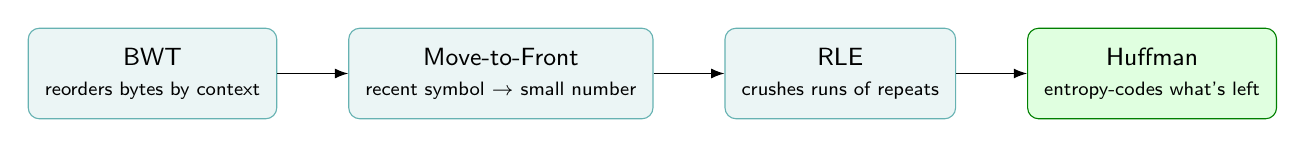
\begin{tikzpicture}[
  box/.style={draw, rounded corners, align=center, font=\sffamily\small, inner sep=6pt, minimum height=1.15cm},
  >=Latex
]
\node[box, fill=teal!8, draw=teal!60] (bwt) {BWT\\{\scriptsize reorders bytes by context}};
\node[box, fill=teal!8, draw=teal!60, right=9mm of bwt] (mtf) {Move-to-Front\\{\scriptsize recent symbol $\to$ small number}};
\node[box, fill=teal!8, draw=teal!60, right=9mm of mtf] (rle) {RLE\\{\scriptsize crushes runs of repeats}};
\node[box, fill=green!12, draw=green!50!black, right=9mm of rle] (huff) {Huffman\\{\scriptsize entropy-codes what's left}};
\draw[->] (bwt) -- (mtf);
\draw[->] (mtf) -- (rle);
\draw[->] (rle) -- (huff);
\end{tikzpicture}}
\caption{The bzip2 pipeline. BWT is a pure reordering step; MTF and RLE are clean-up steps that turn the reordered data into something almost trivial to compress; Huffman (green, as in Figure~2) does the actual entropy coding.}
\end{figure}

The \textbf{Burrows--Wheeler Transform (BWT)} considers every cyclic rotation of a block of input, sorts those rotations lexicographically, and outputs the last column of the sorted list (along with an index needed to invert the transform). It does not compress anything by itself — the output is the same length as the input — but it has a remarkable property: because the rotations are sorted by what \emph{follows} each character, characters that tend to occur in the same context end up clustered together in runs in the output. Reversing the transform is a clever bit of index bookkeeping that recovers the original string exactly.

\textbf{Move-to-Front (MTF)} then walks through this rearranged data maintaining a list of symbols seen so far; each time a symbol appears, it is reported by its current position in the list and then moved to the front. Because BWT clusters identical/similar symbols together, MTF turns those clusters into long runs of zeros (or very small numbers) — "this symbol was just seen" becomes the overwhelmingly common case.

\textbf{Run-Length Encoding (RLE)} then collapses those runs of repeated small numbers efficiently, and a final \textbf{Huffman} stage entropy-codes whatever's left. bzip2 operates on fixed-size blocks (commonly up to 900 KB); larger blocks generally improve the compression ratio (more context for BWT to exploit) at the cost of more memory.

bzip2 is the clearest illustration in this whole guide that "transform to expose redundancy, then entropy-code the rest" is not just an entropy-coding idea — it's the design philosophy of compression in general. It is the same idea as JPEG (Section~6), just applied to arbitrary bytes instead of pixels.

\section{Context modeling and the research frontier}

\begin{figure}[h]
\centering
\resizebox{0.6\textwidth}{!}{%
\begin{forest}
for tree={
  draw, rounded corners, align=center, l sep+=10pt, s sep+=8pt,
  edge={-{Latex[length=2mm]}}, anchor=north, child anchor=north,
  font=\sffamily\small, inner sep=5pt
}
[Context modeling, fill=gray!10, draw=gray!70
  [PPM\\{\scriptsize blended context orders\\+ arithmetic coding}, fill=teal!8, draw=teal!60]
  [CM / PAQ / cmix\\{\scriptsize dozens of mixed models\\+ arithmetic coding}, fill=green!12, draw=green!50!black]
]
\end{forest}}
\caption{The context-modeling family. Green marks the best known compression ratios of any family in this guide, at the cost of being many orders of magnitude slower than everything else here.}
\end{figure}

A family worth knowing about even though it rarely appears in consumer software: \textbf{Prediction by Partial Matching (PPM)} predicts the next symbol from a blend of several preceding context lengths (e.g., the previous 1, 2, 3, \ldots characters), falling back to shorter contexts when a longer one hasn't been seen before, and feeds those predictions to an arithmetic coder. \textbf{Context mixing (CM)} compressors (the PAQ family, and its descendants like \texttt{cmix}) go further, blending predictions from dozens or hundreds of statistical and even small neural-network models with a final arithmetic coder.

These approaches regularly produce the best compression ratios known for general text and are the basis of long-running benchmarks like the Hutter Prize for text compression, but they can be many orders of magnitude slower than Huffman, LZ77, or even arithmetic coding alone, which is why they remain primarily a research and benchmarking tool rather than something you'd find in a day-to-day archiver. They are worth mentioning in an overview precisely because they mark the opposite end of the spectrum from tANS: maximum ratio, with speed treated as essentially irrelevant.

\section{Lossy compression: transform coding for media}

Lossy compression follows the exact same "transform, then entropy-code" template, with one addition: a \textbf{quantization} step that deliberately discards information that a model of human perception predicts won't be missed. This is where the actual, irreversible loss happens — the transform itself is normally lossless (or nearly so); quantization is the lossy step.

\subsection{Images}

\begin{figure}[h]
\centering
\resizebox{0.95\textwidth}{!}{%
\begin{forest}
for tree={
  draw, rounded corners, align=center, l sep+=10pt, s sep+=6pt,
  edge={-{Latex[length=2mm]}}, anchor=north, child anchor=north,
  font=\sffamily\small, inner sep=5pt
}
[Image codecs, fill=gray!10, draw=gray!70
  [JPEG\\{\scriptsize block DCT}, fill=orange!8, draw=orange!60!black]
  [JPEG2000\\{\scriptsize wavelet}, fill=orange!8, draw=orange!60!black]
  [WebP\\{\scriptsize VP8 intra coding}, fill=orange!8, draw=orange!60!black]
  [AVIF\\{\scriptsize AV1 intra coding}, fill=green!12, draw=green!50!black]
  [HEIC / HEIF\\{\scriptsize HEVC intra coding}, fill=orange!8, draw=orange!60!black]
]
\end{forest}}
\caption{Image codecs. Note that three of the five leaves are not independent image formats at all — they are the intra-frame (single-frame) coding tools of a video codec, repurposed for stills. Green marks AVIF as the strongest ratio of the group at the time of writing.}
\end{figure}

\textbf{JPEG} is the canonical example. The pipeline is: convert the image from RGB to a luma/chroma colour space (YCbCr), optionally subsample the chroma channels at lower resolution than luma (since the eye is far less sensitive to colour detail than to brightness — this is itself a lossy step before the transform even runs), split each channel into 8$\times$8 pixel blocks, apply a \textbf{Discrete Cosine Transform (DCT)} to convert each block from pixel values into a weighted sum of frequency components, \textbf{quantize} those frequency coefficients (dividing by a quantization table tuned by a "quality" setting, which rounds high-frequency detail toward zero since the eye is least sensitive to it), reorder the coefficients in a zig-zag scan to cluster the now-mostly-zero high frequencies together, and finally entropy-code the result with Huffman coding (the original 1992 standard) or, less commonly, arithmetic coding.

\textbf{JPEG2000} follows the same transform-quantize-entropy-code template but replaces the block DCT with a \textbf{wavelet transform} applied to the whole image (or large tiles), which avoids the blocky artefacts classic JPEG can show at low quality and allows a genuinely \emph{lossless} mode using a reversible integer wavelet. Its entropy stage (EBCOT) is also considerably more sophisticated than JPEG's Huffman tables. Despite technical advantages, it never displaced JPEG in mainstream use, largely due to higher computational cost and patent concerns during its rollout.

Newer image formats reuse video-codec technology for still images rather than inventing new transforms: \textbf{WebP} is built on the intra-frame coding tools of the VP8 video codec, \textbf{AVIF} on AV1's intra-frame coding, and \textbf{HEIC/HEIF} on HEVC's intra-frame coding. This is a nice point for a thorough overview: by the 2010s, video codecs had become such good general-purpose image compressors (because a video frame is just an image, and codecs spend enormous engineering effort compressing those well) that it became more efficient to reuse them for stills than to design new still-image formats from scratch.

\subsection{Audio}

\begin{figure}[h]
\centering
\resizebox{0.85\textwidth}{!}{%
\begin{forest}
for tree={
  draw, rounded corners, align=center, l sep+=10pt, s sep+=6pt,
  edge={-{Latex[length=2mm]}}, anchor=north, child anchor=north,
  font=\sffamily\small, inner sep=5pt
}
[Audio codecs, fill=gray!10, draw=gray!70
  [Lossy\\{\scriptsize MDCT + psychoacoustic model}, fill=orange!12, draw=orange!70!black
    [MP3, fill=orange!8, draw=orange!60!black]
    [AAC, fill=orange!8, draw=orange!60!black]
    [Opus, fill=green!12, draw=green!50!black]
  ]
  [Lossless\\{\scriptsize linear prediction + Rice coding}, fill=teal!10, draw=teal!70
    [FLAC, fill=teal!8, draw=teal!60]
    [ALAC, fill=teal!8, draw=teal!60]
  ]
]
\end{forest}}
\caption{Audio codecs split the same way the whole field does (Figure~1): lossy formats trade fidelity for size using a psychoacoustic model, lossless formats use prediction and Rice coding to recover the exact waveform. Green marks Opus as the most modern, latency-flexible option.}
\end{figure}

Lossy audio compression replaces the spatial DCT/wavelet with a transform over \emph{time}, almost always a \textbf{Modified Discrete Cosine Transform (MDCT)}, and replaces "the eye is less sensitive to fine colour/high spatial frequency" with a \textbf{psychoacoustic model} of what the human ear can and cannot perceive — in particular, masking effects, where a loud sound at one frequency makes nearby frequencies and immediately following moments effectively inaudible. Coefficients in masked regions can be quantized far more coarsely, or dropped entirely, without an audible difference.

\textbf{MP3} (MPEG-1 Audio Layer III) was the format that brought this to the mainstream, using MDCT plus a psychoacoustic model plus Huffman coding. \textbf{AAC} improves on MP3 with better transform and prediction tools and is the default lossy audio codec in most modern streaming and mobile platforms. \textbf{Opus} is a more recent, low-latency codec (a hybrid of the SILK speech codec and the CELT transform codec) designed for real-time use such as voice calls and live streaming, where MP3/AAC's larger encoding delay is a problem.

Not every audio codec is lossy: \textbf{FLAC} and Apple's \textbf{ALAC} are \emph{lossless} audio codecs — they use linear prediction (predicting each sample from previous ones) followed by an entropy coder (commonly Rice/Golomb coding, a simple and very fast entropy code well-suited to the geometrically-distributed prediction residuals audio tends to produce) and recover the exact original waveform, at roughly half the size of uncompressed audio rather than MP3/AAC's much larger reductions.

\subsection{Video}

\begin{figure}[h]
\centering
\resizebox{0.95\textwidth}{!}{%
\begin{forest}
for tree={
  draw, rounded corners, align=center, l sep+=10pt, s sep+=6pt,
  edge={-{Latex[length=2mm]}}, anchor=north, child anchor=north,
  font=\sffamily\small, inner sep=5pt
}
[Video codecs, fill=gray!10, draw=gray!70
  [Licensed standards, fill=orange!12, draw=orange!70!black
    [MPEG-2, fill=orange!8, draw=orange!60!black]
    [H.264 / AVC, fill=orange!8, draw=orange!60!black]
    [H.265 / HEVC, fill=orange!8, draw=orange!60!black]
    [VVC / H.266, fill=orange!8, draw=orange!60!black]
  ]
  [Royalty-free, fill=orange!12, draw=orange!70!black
    [VP9, fill=orange!8, draw=orange!60!black]
    [AV1, fill=green!12, draw=green!50!black]
  ]
]
\end{forest}}
\caption{Video codecs grouped by licensing model as much as by technology — patent and royalty considerations have shaped adoption almost as strongly as compression ratio. Green marks AV1 as the current state of the art among the royalty-free options.}
\end{figure}

Video compression adds one more redundancy to exploit beyond what images have: most of the time, the next frame looks a lot like the previous one. Video codecs add \textbf{motion estimation and compensation}: rather than transform-coding every frame from scratch, the encoder finds which block of the previous (reference) frame each block of the current frame most closely matches, after a small motion shift, and only needs to transmit that motion vector plus a (typically small) residual difference. Frames are categorized as \textbf{I-frames} (independently coded, like a still image), \textbf{P-frames} (predicted from previous frames), and \textbf{B-frames} (predicted from both previous and future frames). The residual after motion compensation still goes through the same block-transform-quantize-entropy-code pipeline as a still image, plus an in-loop filtering step (e.g., deblocking) to smooth block artefacts before the frame is used as a reference for the next one.

The entropy stage is where Section~4's coders reappear directly: H.264 offers a choice between CAVLC (a Huffman-style scheme) and CABAC (context-adaptive binary arithmetic coding) for the final stage, with CABAC giving meaningfully better compression at higher computational cost.

The major standards, roughly in order of adoption:
\begin{itemize}[leftmargin=1.4em]
  \item \textbf{MPEG-2} — broadcast television and DVDs; the baseline most later standards improved on.
  \item \textbf{H.264 / AVC} (2003) — by far the most widely deployed video codec in history; still the safe, universally-supported default.
  \item \textbf{H.265 / HEVC} (2013) — roughly 50\% better compression than H.264 at the same quality, used heavily for 4K streaming, but encumbered by a more complicated patent licensing landscape that slowed adoption.
  \item \textbf{VP9} (Google, 2013) — a royalty-free competitor to HEVC, used extensively by YouTube.
  \item \textbf{AV1} (Alliance for Open Media, 2018) — a royalty-free, jointly-developed successor to VP9 with compression efficiency competitive with or better than HEVC; the current state of the art for major streaming platforms (YouTube, Netflix).
  \item \textbf{VVC / H.266} (2020) — the newest standardized codec, aiming for roughly another 50\% improvement over HEVC, still in early deployment.
\end{itemize}

\section{A complete reference table}

The table below collects every algorithm mentioned in this guide in one place, for quick reference after watching the video.

\begin{longtable}{@{}L{3.0cm}L{2.6cm}L{1.4cm}L{4.0cm}L{4.0cm}@{}}
\toprule
\textbf{Algorithm} & \textbf{Family} & \textbf{Lossy?} & \textbf{Typical use} & \textbf{Defining trait} \\
\midrule
\endhead
Huffman coding & Entropy (prefix) & No & DEFLATE, classic JPEG & Optimal among whole-bit prefix codes \\
Shannon--Fano & Entropy (prefix) & No & Historical & Precursor to Huffman, slightly suboptimal \\
Arithmetic coding & Entropy (non-prefix) & No & PAQ-family, some video modes & Reaches the entropy limit; slow \\
Range coding & Entropy (non-prefix) & No & LZMA / 7-Zip / xz & Byte-oriented reformulation of arithmetic coding \\
rANS & Entropy (ANS) & No & Modern codecs & Fast, parallel-friendly state transform \\
tANS / FSE & Entropy (ANS) & No & Zstandard, LZFSE & Table-driven; fastest entropy coder in common use \\
CABAC & Entropy (context-adaptive) & No$^{*}$ & H.264, HEVC & Context-adaptive binary arithmetic coding \\
LZ77 & Dictionary & No & Foundational & Sliding-window match-and-copy \\
LZ78 / LZW & Dictionary & No & GIF, \texttt{compress} & Explicit growing dictionary \\
DEFLATE & Dictionary + entropy & No & \texttt{.zip}, gzip, PNG & LZ77 + Huffman \\
LZMA & Dictionary + entropy & No & 7-Zip, \texttt{.xz} & LZ77 + range coding, large window \\
Zstandard (zstd) & Dictionary + entropy & No & General-purpose (Meta) & LZ77 + tANS/FSE, tunable speed/ratio \\
LZ4 & Dictionary & No & Real-time systems & No entropy stage; extreme decode speed \\
Snappy & Dictionary & No & Google infrastructure & Speed prioritized over ratio \\
Brotli & Dictionary + entropy & No & Web (HTTP compression) & Static web-content dictionary + Huffman \\
bzip2 (BWT pipeline) & Transform & No & General-purpose archiving & BWT + MTF + RLE + Huffman \\
PPM & Context modeling & No & Text compression research & Blended multi-order context prediction \\
CM / PAQ / cmix & Context modeling & No & Research, Hutter Prize & Best known ratios; extremely slow \\
JPEG & Transform (DCT) & Yes & Photographs & Block DCT + quantization + Huffman \\
JPEG2000 & Transform (wavelet) & Yes / No mode & Cinema, medical imaging & Wavelet transform + EBCOT \\
WebP & Transform (video intra) & Yes / No mode & Web images & Built on VP8 intra-frame coding \\
AVIF & Transform (video intra) & Yes / No mode & Modern web images & Built on AV1 intra-frame coding \\
HEIC / HEIF & Transform (video intra) & Yes / No mode & iPhone photos & Built on HEVC intra-frame coding \\
MP3 & Transform + psychoacoustic & Yes & Legacy audio & MDCT + masking model + Huffman \\
AAC & Transform + psychoacoustic & Yes & Streaming, mobile audio & Improved transform/prediction over MP3 \\
Opus & Transform + psychoacoustic & Yes & VoIP, live streaming & Low-latency hybrid (SILK + CELT) \\
FLAC / ALAC & Predictive & No & Audio archiving & Linear prediction + Rice coding \\
MPEG-2 & Transform + motion & Yes & Broadcast TV, DVD & Early block-motion video standard \\
H.264 / AVC & Transform + motion & Yes & Most-deployed video codec & CAVLC/CABAC back-end \\
H.265 / HEVC & Transform + motion & Yes & 4K streaming & $\sim$50\% better than H.264 \\
VP9 & Transform + motion & Yes & YouTube & Royalty-free HEVC competitor \\
AV1 & Transform + motion & Yes & YouTube, Netflix & Royalty-free, state of the art \\
VVC / H.266 & Transform + motion & Yes & Emerging & Newest standard, early deployment \\
\bottomrule
\end{longtable}
\noindent\footnotesize $^{*}$CABAC itself is lossless; it is the final stage of codecs whose overall pipeline is lossy.\normalsize

\section{The unifying takeaway}

Every algorithm in this guide, lossless or lossy, simple or state-of-the-art, is some combination of two ingredients: \textbf{a model or transform that exposes redundancy}, and \textbf{an entropy coder that spends fewer bits on the predictable parts}. Huffman coding, arithmetic coding, and the ANS family are different answers to "how close can we get to the entropy limit, and how fast?" LZ77, LZMA, and Zstandard are different answers to "how do we expose redundancy by finding repeated chunks?" BWT and PPM are different answers to "how do we expose redundancy by reorganizing or predicting?" And JPEG, MP3, and AV1 are different answers to "given that we're allowed to throw a little information away, where should that come from, and how do we entropy-code what's left?"

Once that pattern is visible, the field stops looking like a long list of unrelated acronyms and starts looking like a small number of ideas, recombined.

\end{document}
